\newpage
\subsubsection*{7.}
On va afficher les attributs des tables thing et subscribe en utilisant la table
USER\_TAB\_COLUMNS depuis DBAIOT , en va afficher le nom , id , type , longeur de chaque attributs
et on fait un WHERE table\_name='THING' pour afficher les attributs de la table THING puis WHERE table\_name='SUBSCRIBE' 
pour les attributs de la table SUBSCRIBE

\subsubsection*{7.a}

\lstinputlisting[style=sqlstyle]{SQL/Partie5/thing.sql}

\begin{center}
    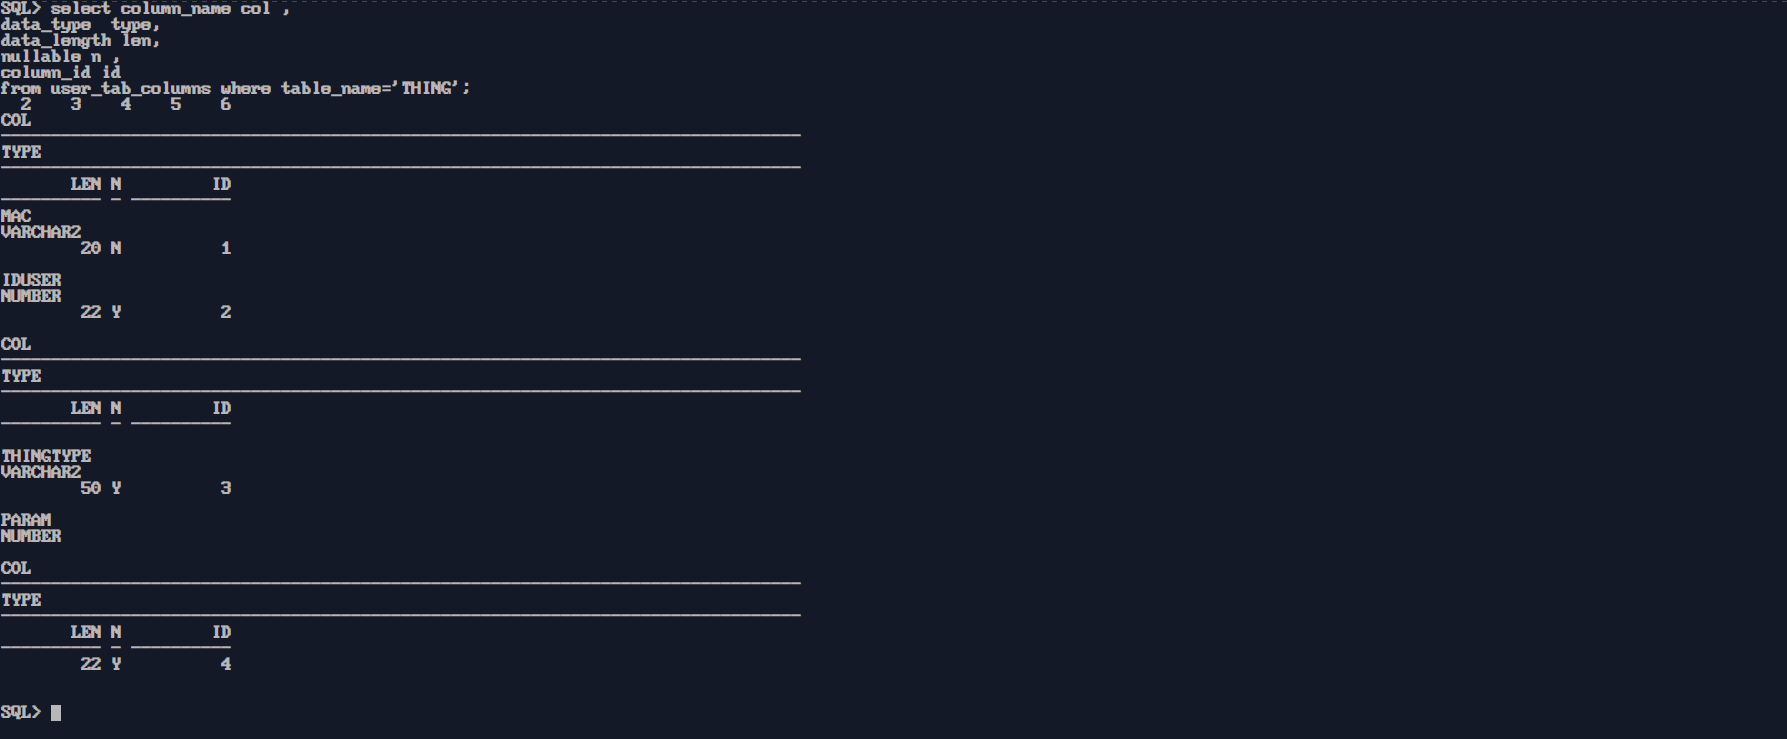
\includegraphics[width=\textwidth]{ScreenShot/Partie5/thing.png}
\end{center}


\subsubsection*{7.b}

\lstinputlisting[style=sqlstyle]{SQL/Partie5/sub.sql}

\begin{center}
    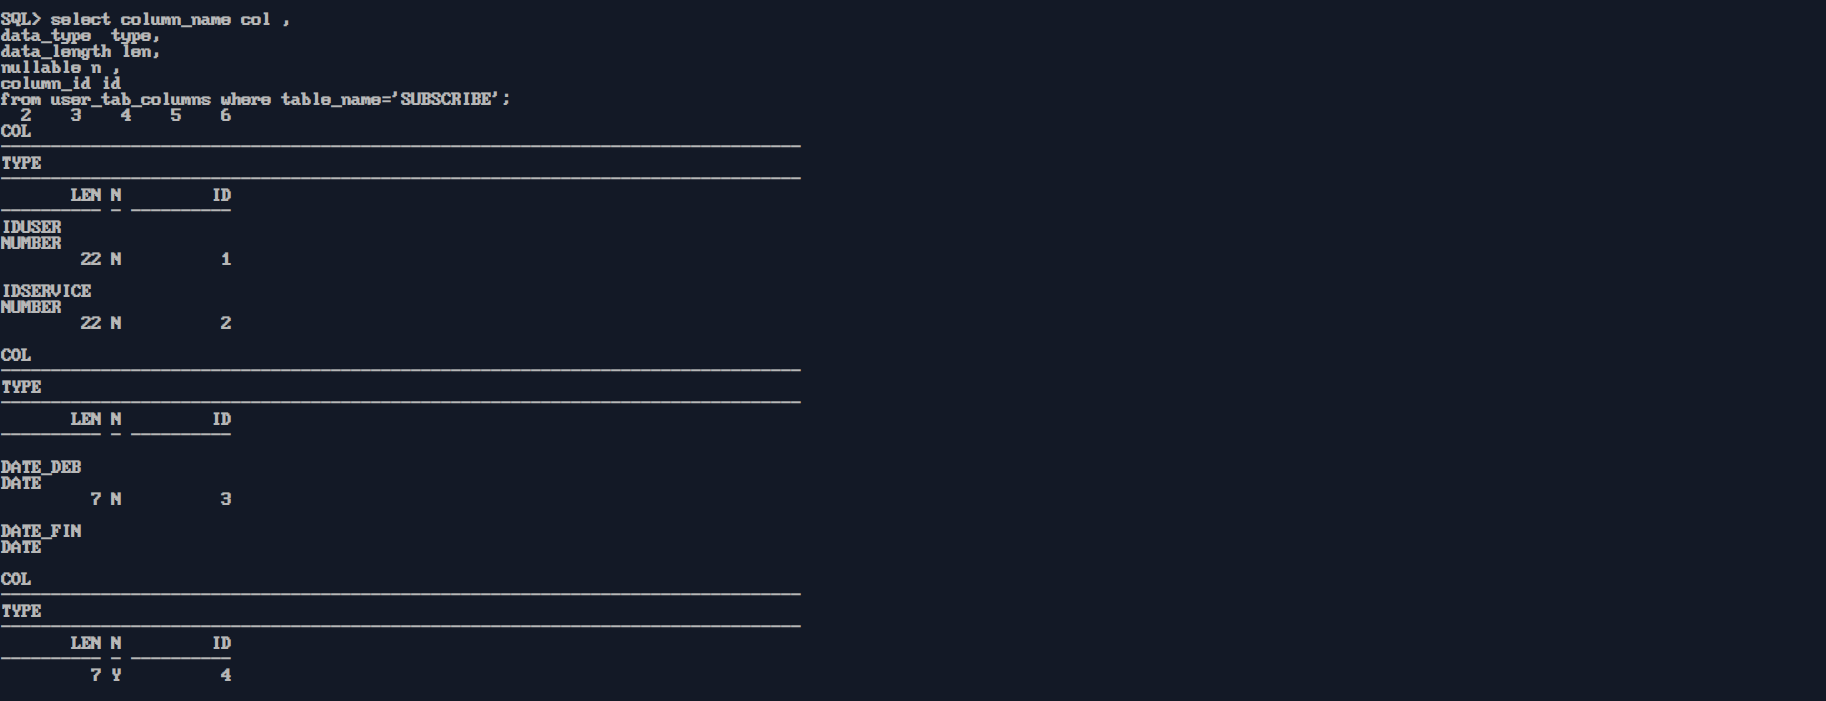
\includegraphics[width=\textwidth]{ScreenShot/Partie5/sub.png}
\end{center}

